% Introduzione
\chapter{Introduzione}\label{ch:introduzione}
Il lavoro di tesi è stato realizzato in collaborazione con Magenta srl \cite{magenta} e con l'Istituto per la BioEconomia del Consiglio Nazionale delle Ricerche (IBE CNR) \cite{ibe}.\\

L'oggetto di studio è la piattaforma AirQino \cite{airqino} per il monitoraggio ambientale ad alta precisione in ambito urbano. Gli obiettivi sono stati molteplici:
\begin{itemize}
  \item Sviluppi tecnologici alla piattaforma, rivolti a migliorare in un caso l'affidabilità dei dati inviati dai sensori, e nell'altro la gestione del problema della quantità di dati in aumento costante (capitolo \ref{ch:sviluppi});
  \item Studio e analisi del processo di calibrazione delle centraline AirQino, con un confronto quantitativo sulle diverse procedure utilizzate (capitolo \ref{ch:calibrazione});
  \item Realizzazione di un'interfaccia che permetta la calibrazione di più centraline contemporaneamente  (capitolo \ref{ch:interfaccia}).
\end{itemize}

\begin{figure}[H]
\centering
\captionsetup{justification=centering}

\includegraphics[width=0.65\textwidth,height=\textheight,keepaspectratio]{img/magenta}
\caption{Magenta srl\\Fonte: \url{https://magentalab.it}}
\label{fig:magenta}
\end{figure}

\begin{figure}[H]
\centering
\captionsetup{justification=centering}

\includegraphics[width=0.75\textwidth,height=\textheight,keepaspectratio]{img/ibe.jpg}
\caption{CNR - Istituto per la BioEconomia (IBE)\\Fonte: \url{https://www.ibe.cnr.it}}
\label{fig:ibe}
\end{figure}

\begin{figure}[H]
\centering
\captionsetup{justification=centering}

\includegraphics[width=0.60\textwidth,height=\textheight,keepaspectratio]{img/airqino}
\caption{La piattaforma AirQino\\Fonte: \url{https://airqino.it}}
\label{fig:airqino}
\end{figure}

% Contesto
\section{Contesto}\label{sec:contesto}
Il monitoraggio della qualità dell'aria è una delle attività più importanti per la tutela della salute pubblica. La qualità dell'aria può essere influenzata da molte sorgenti di emissione, tra cui le automobili, le centrali elettriche, gli impianti di riscaldamento e le fabbriche. I principali inquinanti atmosferici sono il biossido di zolfo, gli idrocarburi policiclici aromatici, il monossido di carbonio e gli ozono. Gli effetti dell'inquinamento atmosferico sulla salute sono molteplici e possono essere a breve o a lungo termine. I principali rischi sono l'asma, le malattie cardiovascolari, il cancro e le malattie respiratorie. Il monitoraggio della qualità dell'aria permette di individuare le sorgenti di emissione e di intervenire per ridurre l'inquinamento atmosferico.

\subsection{Descrizione del problema}\label{ssec:problema}
\ldots

\subsection{Motivazioni}\label{ssec:motivazoni}
\ldots

% La piattaforma AirQino
\section{La piattaforma AirQino}\label{sec:airqino}

% todo riferimenti
AirQino è una piattaforma di monitoraggio ambientale ad alta precisione, realizzata dal Consiglio Nazionale delle Ricerche (CNR) in collaborazione con TEA Group e Quanta Srl. \cite{GUALTIERI2017609}

Il progetto nasce dall’esigenza di realizzare una rete di stazioni mobile per un monitoraggio più completo della qualità dell’aria in ambito urbano, in linea con la direttiva europea 2008/50/EC \cite{direttiva}, che riconosce e regolamenta l’importanza di misure aggiuntive rispetto a quelle delle stazioni fisse.

Alcune delle caratteristiche di AirQino sono:
\begin{itemize}
  \item Sistema di rilevamento \textbf{polifunzionale}: il sistema offre la possibilità di rilevare gli agenti inquinanti presenti in atmosfera e identificarne le sorgenti;
  \item Sistema \textbf{versatile} e dispiegabile in più punti per creare una rete di monitoraggio capillare, flessibile ed economica;
  \item Alte \textbf{prestazioni} dei sensori installati, garantite da una rigorosa calibrazione e validazione degli apparati da parte dei laboratori del CNR;
  \item Tutte le stazioni sono \textbf{configurabili} con un’ampia gamma di sensori aggiuntivi a seconda delle proprie esigenze.
\end{itemize}

\begin{figure}[H]
\centering
\captionsetup{justification=centering}
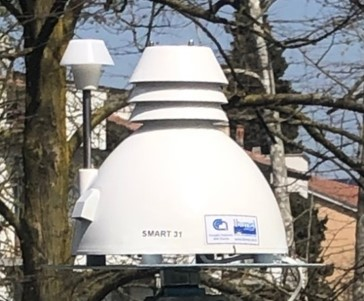
\includegraphics[width=0.50\textwidth,height=\textheight,keepaspectratio]{img/airqino_stazione}
\caption{Una centralina AirQino\\Fonte: \url{https://airqino.it}}
\label{fig:airqino_stazione}
\end{figure}

La rete di sensori AirQino consente rilevare le principali sostanze inquinanti riscontrabili nell’aria (\ce{NO2}, \ce{O3}, \ce{CO}, \ce{PM_{2.5}}, \ce{PM_{10}}) ma anche ulteriori parametri ambientali, come la temperatura, l'umidità relativa dell’aria e il principale gas climalterante, la \ce{CO2} (tabella \ref{fig:sensori-airqino}).
Inoltre la centralina è estendibile, e permette di aggiungere ulteriori sensori ausiliari in base alle preferenze.

\begin{table}[H]
    \footnotesize
    \centering
    \def\arraystretch{0.9}
    \begin{tabular}{|l|l|l|l|l|l|}
    \hline
        \textbf{Sensori} & \textbf{Tipologia} & \textbf{Unità} & \textbf{Range} & \textbf{Prec.} \\ \hline
        \ce{NO2} & Sensori di gas MOS & $\mathrm{\si{\micro}g/m^3}$ & 0-5000 & 15\% \\ \hline
        \ce{O3} & Semiconduttore & $\mathrm{\si{\micro}g/m^3}$ & 0-1000 & 15\% \\ \hline
        CO & Sensori di gas MOS & $\mathrm{\si{\micro}g/m^3}$ & 0-30 & 15\% \\ \hline
        VOC totali & Sensori di gas MOS & $\mathrm{\si{\micro}g/m^3}$ & 0-1000 & 15\% \\ \hline
        \ce{CO2} & NDIR & ppm o $\mathrm{\si{\micro}g/m^3}$ & 0-2000 & 10\% \\ \hline
        \ce{PM_{2.5}} & Contatore di particelle ottico & $\mathrm{\si{\micro}g/m^3}$ & 0-1000 & 10\% \\ \hline
        \ce{PM10} & Contatore di particelle ottico & $\mathrm{\si{\micro}g/m^3}$ & 0-1000 & 10\% \\ \hline
        Umidità relativa & Stato solido & \% & 0-100 & 5\% \\ \hline
        Temp. dell’aria & Stato solido & °C & -40 - 80 & 5\% \\ \hline
        Temp. interna & Stato solido & °C & -40 - 80 & 5\% \\ \hline
    \end{tabular}
    \caption{Tipologie di sensori in dotazione con le centraline AirQino (configurazione base, estendibile). Fonte: \url{https://airqino.it}}
    \label{fig:sensori-airqino}
\end{table}

Lato frontend, la pagina si apre su mappa interattiva che visualizza tutte le reti di centraline. Selezionata una stazione di interesse, vengono mostrati dettagli e foto della stazione stessa (figura \ref{fig:airqino}). Per ciascun sensore della centralina selezionata è possibile visualizzare grafici di andamento medio settimanali, insieme al dato istantaneo relativo all'ultima misurazione.

\begin{figure}[H]
\centering
\captionsetup{justification=centering}
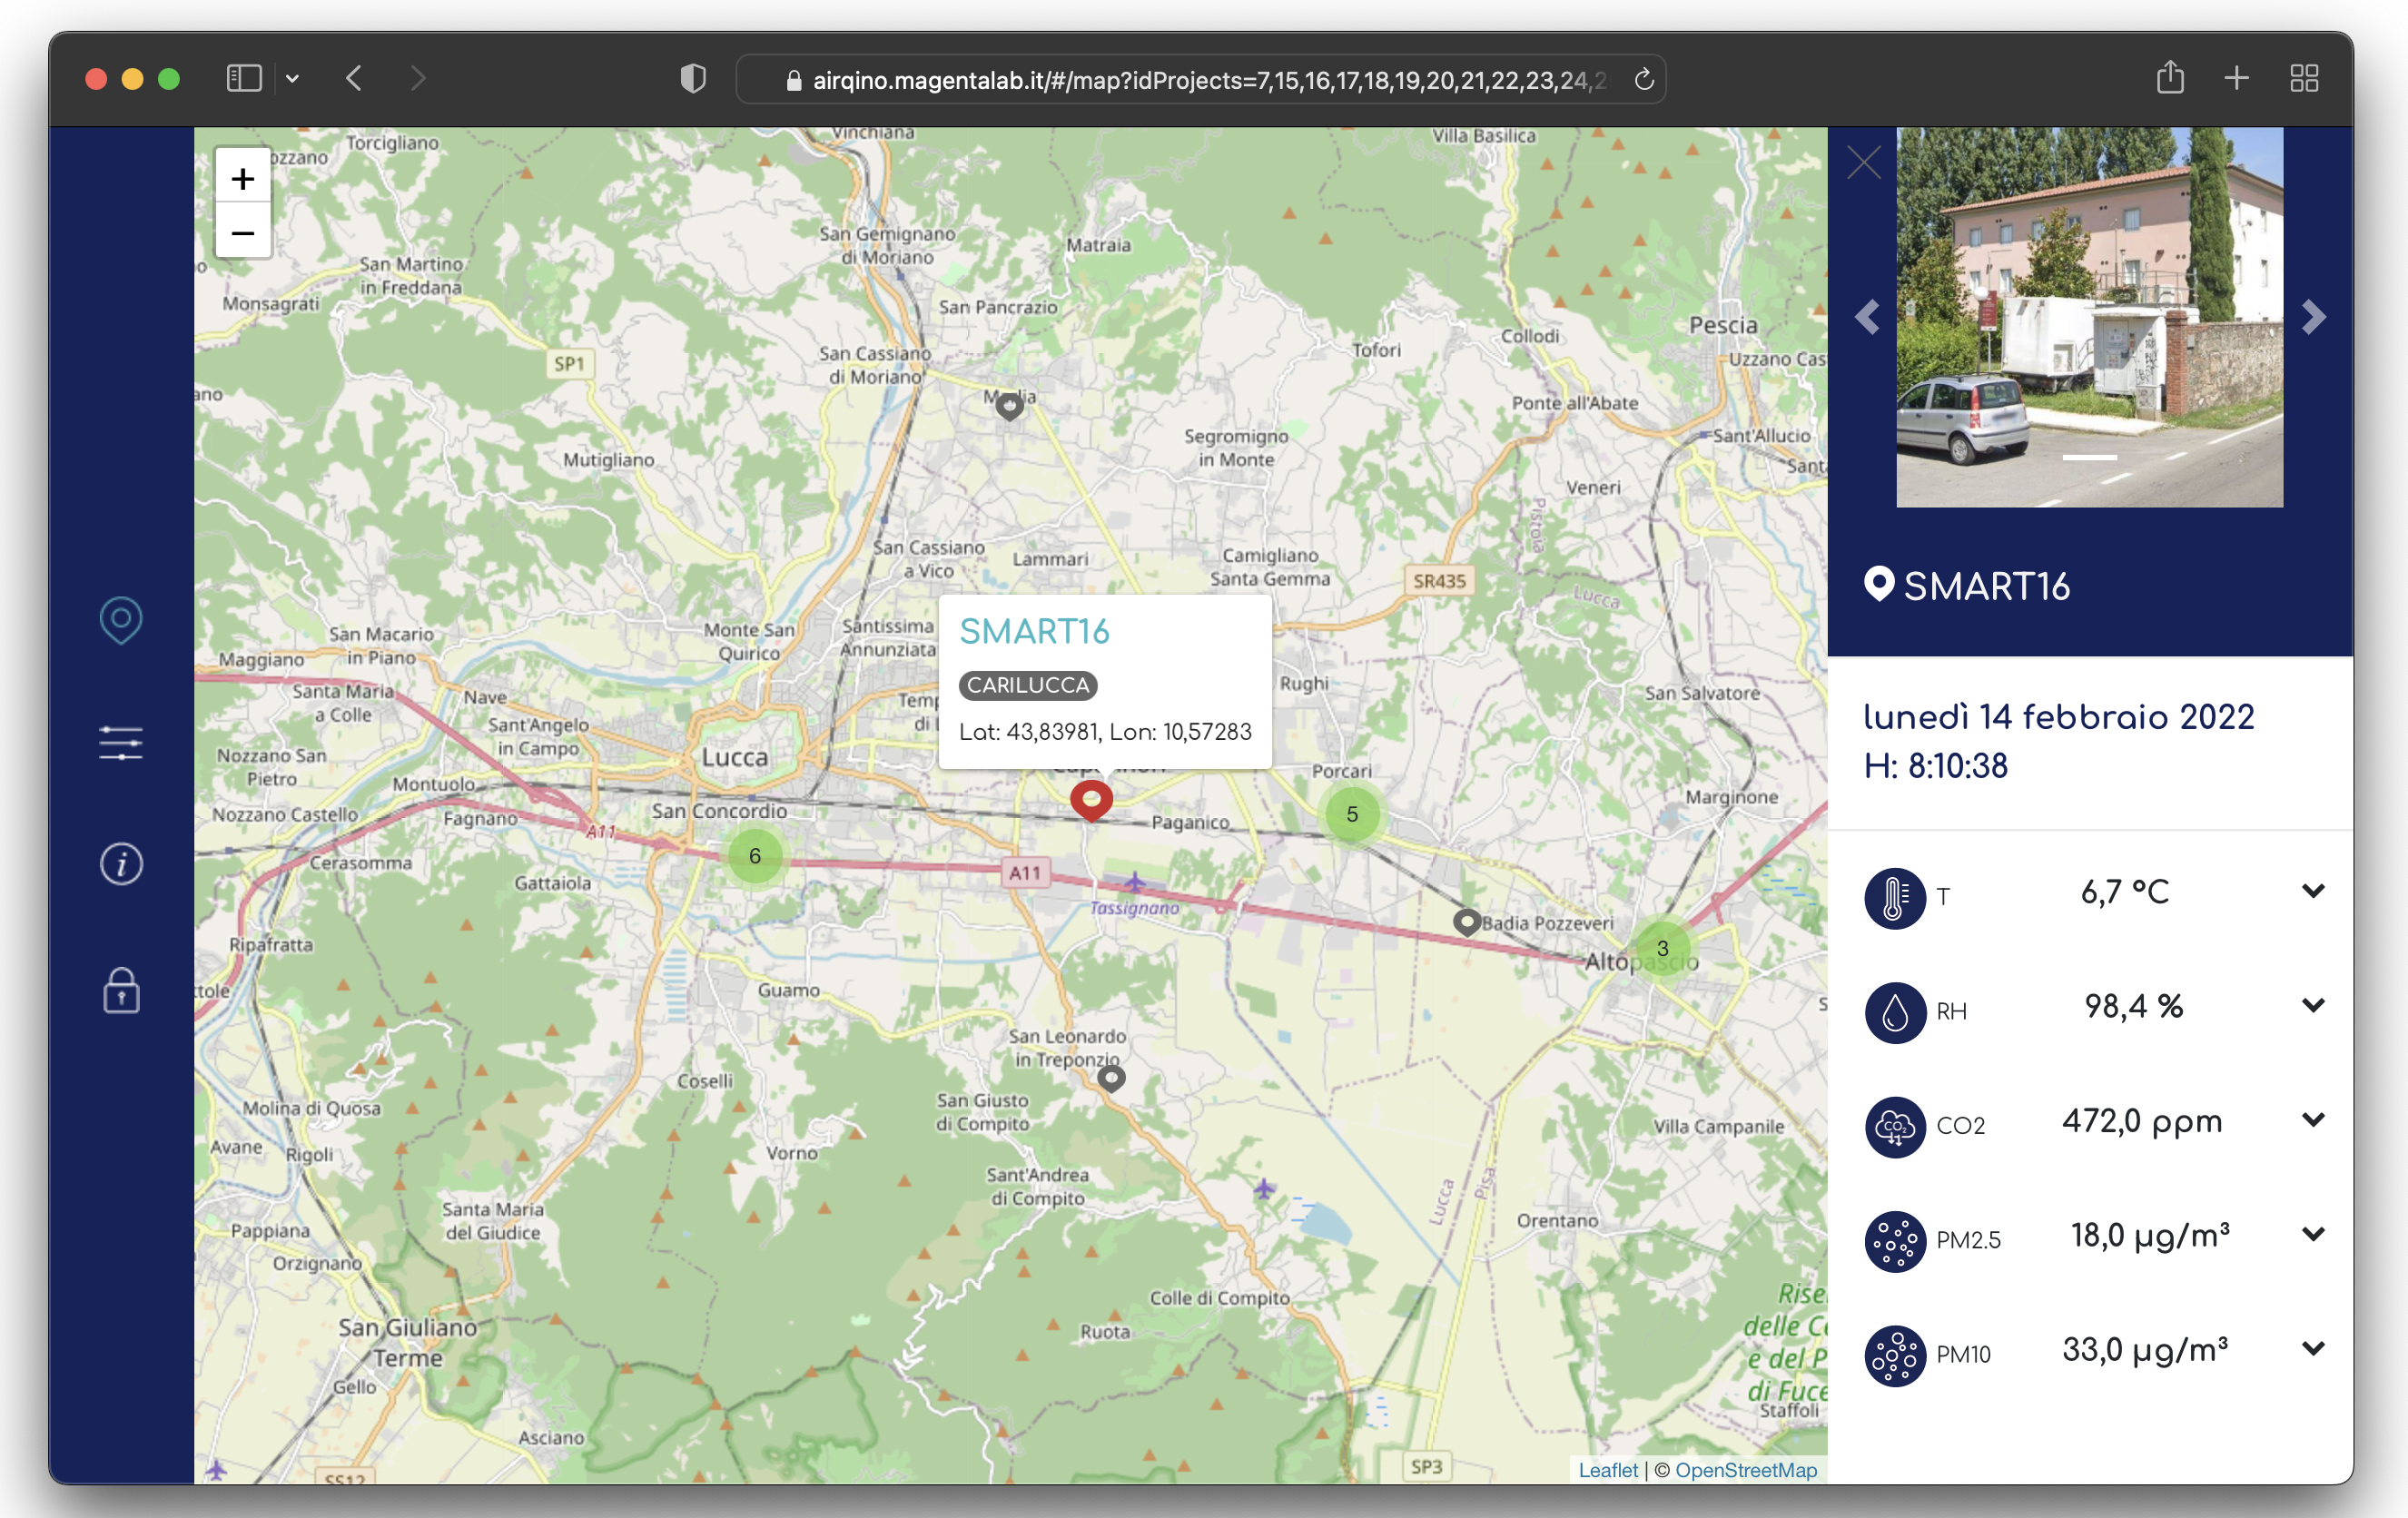
\includegraphics[width=0.70\textwidth,height=\textheight,keepaspectratio]{img/airqino_web}
\caption{La piattaforma web di AirQino\\Fonte: \url{https://airqino.magentalab.it}}
\label{fig:airqino}
\end{figure}

\subsection{Architettura e tecnologie}\label{ssec:airqino-architettura}
Il sistema è composto dai seguenti elementi principali:

\begin{itemize}
  \item \textbf{Gateway}: server che espone servizi compatibili con le centraline, e normalizza i dati trasmessi verso il server di raccolta. Questa applicazione, realizzata con Java e framework \textbf{Spring} \cite{spring}, fornisce un endpoint con lo stesso indirizzo a cui le centraline comunicano, in modo da garantire continuità di servizio. Il gateway ha anche il compito di segnalare eventuali interruzioni di funzionamento, secondo regole ben definite. Il gateway produce anche un output su protocollo \textit{MQTT2}, utilizzando un broker open source per pubblicare i dati verso il backend;
  \item \textbf{Backend}: applicazione server che si interfaccia con il broker \textit{MQTT} e scrive sul database i dati, esponendo inoltre servizi web di tipo REST utilizzati dal frontend web. Il backend è realizzato con Java e framework \textbf{Spring} \cite{spring} e utilizza \textbf{Timescale} \cite{timescale}, un database relazionale open source per la gestione efficienti di dati temporali;
  \item \textbf{Frontend}: applicazione web che permette la visualizzazione di mappa e grafici dei dati raccolti dalle centraline, utilizzando i servizi esposti dal backend. L'interfaccia è basata su tecnologia \textbf{Angular} \cite{angular}. Il frontend ha anche una sezione \textit{admin}, protetta da autenticazione, che permette la gestione del sistema. Le funzionalità di gestione previste sono:
    \begin{itemize}
      \item Gestione anagrafica centraline (nome, posizione, progetti a cui afferisce);
      \item Configurazione dei parametri di funzionamento tra cui i parametri di calibrazione, per la trasformazione da dati grezzi a valori leggibili dall’utente, e le soglie rilevamento allarmi;
      \item Gestione utenti;
      \item Scaricamento dati raw oppure convertiti.
    \end{itemize}
\end{itemize}

\subsection{Hardware dei sensori}\label{ssec:hardware}
% todo schematics
Per quanto riguarda la caratteristiche dei sensori, i sensori di tipo MOS sono costituiti da un film (credo allumina? Per  fabbricare  gli  strati  sensibili  del  film,  si  prepara  una  pasta  viscosa:  al  materiale funzionale,  sotto  forma  di  polvere,  viene  aggiunta  una  miscela  di  agenti  reologici  in  solventi  volatili) depositato su una piastra di elementi riscaldanti la cui temperatura operativa è generalmente compresa tra 300 e 500°C. Di solito il  materiale funzionale del film più  adatto per  la  rilevazione di  biossido  di  azoto è l’ossido  di  ferro  e lantanio (LaFeO3) che oltre ad avere una buona sensibilità agli ossidi di azoto ha una  bassa  sensibilità  al  monossido  di  carbonio. Per la rilevazione dell’ozono viene invece utilizzato  triossido di tungsteno (WO3). Questo tipo  di  materiale  funzionale risulta  molto  sensibile  ai  gas  ossidanti  come  O3 e  NO2. Qualsiasi sia il materiale funzionale, il principio di funzionamento per tutti i MOS nella rilevazione di gas è quello di interagire con il gas presente all’interno dell’atmosfera tramite reazioni di ossidoriduzione, portando a un cambiamento di conduttività, che viene rilevato da un circuito apposito. Le variazioni della conduttività dei sensori è fortemente influenzata dalle variazioni di umidità e temperatura, come rilevato dalla letteratura sull'argomento [ref]. Nel caso dei sensori Mics che noi utilizziamo, il produttore non rilascia informazioni sull'influenza nella lettura dovuto alla temperatura/umidità  ma che queste influiscono può essere ipotizzato come può essere ipotizzato che ci sia una influenza introdotta dalla temperatura nel circuito ADC del microcontrollore.

Questo segnale viene passato al convertitore analogico digitale del controllore che lo trasforma in counts (10 bit da 0 a 2 alla 10).

ossidoriduzione → piastra che si scalda a seconda dell'inquinante genera corrente

il segnale viene passato attraverso un convertitore analogico digitale e l’uscita è a 10 bit (questa unità la chiamo counts)

\subsection{Progetti correlati}\label{ssec:correlati}
Di seguito sono elencati alcuni progetti che fanno uso delle centraline AirQino:

\begin{itemize}
  \item \textbf{Prato Urban Jungle} \cite{urbanjungle} mira a promuovere la progettazione urbana creativa e visionaria per ri-naturalizzare i quartieri di Prato in modo sostenibile e socialmente inclusivo;
  \item \textbf{SMART Treedom} \cite{smartreedom} è il frutto dalla collaborazione tra Treedom e l’Istituto di Biometeorologia del Consiglio Nazionale delle Ricerche. La finalità del progetto è stata quella di prototipare un sistema integrato che possa essere modulato con diversi sensori in base al tipo di grandezza fisica che si vuole misurare e una tecnologia laser per la misura delle polveri sottili;
  \item \textbf{Trafair} \cite{trafair} è un progetto europeo biennale co-finanziato dal programma europeo Connecting Europe Facility (CEF) nel settore delle telecomunicazioni con lo scopo di sviluppare un servizio di previsione della qualità dell’aria urbana basata su previsioni meteo e flussi di traffico in sei città europee di dimensioni diverse: Zaragoza, Firenze, Modena, Livorno, Santiago de Compostela e Pisa.
  \item \textbf{Smart Garda Lake} \cite{garda} nasce nel 2017 con lo scopo di creare una rete di monitoraggio ambientale per rilevamenti in campo meteorologico, inquinamento acustico, stato delle acque superficiali e qualità dell’aria all’insegna degli obiettivi di sostenibilità dell’Agenda 2030 dell’ONU;
  \item \textbf{Brenner LEC} \cite{lec} si colloca nel contesto di un’area sensibile come le Alpi e si pone l’obiettivo di creare un “corridoio a emissioni ridotte” (LEC – Lower Emission Corridor) lungo l’asse autostradale del Brennero al fine di ottenere un chiaro beneficio ambientale nei settori della tutela dell’aria e della protezione del clima, nonché una riduzione dell’inquinamento acustico.
\end{itemize}

\subsection{Progetti simili}\label{ssec:competitor}
Ci sono anche altre piattaforme simili ad AirQino:

\begin{itemize}
	\item \textbf{Airly} \cite{airly} è una piattaforma che consente di condividere informazioni ambientali in tempo reale, grazie alla quale è possibile monitorare la qualità dell'aria e i livelli di inquinamento;
	\item \textbf{Aqicn} \cite{aqicn} è un progetto open source lanciato nel 2010 che consente di monitorare l'inquinamento atmosferico in tempo reale;
	\item \textbf{IQAir} \cite{iqair} è una società svizzera che produce e vende purificatori d'aria per uso residenziale e commerciale. La loro applicazione fornisce un rapporto in tempo reale sulla qualità dell'aria e previsione dell'inquinamento atmosferico;
	\item \textbf{Decentlab} \cite{decentlab} è un'azienda svizzera che fornisce dispositivi e servizi di sensori wireless per soluzioni di monitoraggio distribuite ed economiche;
	\item \textbf{PlanetWatch} \cite{planetwatch} è una piattaforma decentralizzata che consente di monitorare e proteggere il pianeta attraverso la condivisione di informazioni. Gli utenti possono condividere informazioni sull'ambiente, la sostenibilità e la responsabilità sociale;
	\item \textbf{HackAIR} \cite{hackair} è una piattaforma open source che consente ai cittadini di monitorare la qualità dell'aria nei propri quartieri. Gli utenti possono interagire con la piattaforma per segnalare la qualità dell'aria nel proprio quartiere, visualizzare i dati relativi alla qualità dell'aria e condividere informazioni e dati con altri utenti.
\end{itemize}
